\documentclass[11pt]{article}
\usepackage{amsmath,amsfonts,latexsym,graphicx}
\usepackage{fullpage}
\usepackage{url,hyperref}
\usepackage{subfig}
\usepackage{tikz}
\usetikzlibrary{arrows,decorations.pathmorphing,backgrounds,fit,shapes.geometric}
\usepgflibrary{shapes.geometric}
%\usepackage{ijcai09}

\pagestyle{empty}

\setlength{\oddsidemargin}{0in}
\setlength{\topmargin}{0in}
\setlength{\textwidth}{6.5in}
\setlength{\textheight}{8.5in}

\newtheorem{fact}{Fact}[section]
\newtheorem{lemma}{Lemma}[section]
\newtheorem{theorem}[lemma]{Theorem}
\newtheorem{assumption}[lemma]{Assumption}
\newtheorem{definition}[lemma]{Definition}
\newtheorem{corollary}[lemma]{Corollary}
\newtheorem{prop}[lemma]{Proposition}
\newtheorem{claim}[lemma]{Claim}
\newtheorem{remark}[lemma]{Remark}
\newtheorem{prob}{Problem}
\newtheorem{conjecture}{Conjecture}


\newenvironment{proof}{\vspace{-0.15in}\noindent{\bf Proof:}}%
        {\hspace*{\fill}$\Box$\par}
\newenvironment{proofsketch}{\noindent{\bf Proof Sketch.}}%
        {\hspace*{\fill}$\Box$\par\vspace{4mm}}
\newenvironment{proofof}[1]{\smallskip\noindent{\bf Proof of #1.}}%
        {\hspace*{\fill}$\Box$\par}

\newcommand{\etal}{{\em et al.}\ }
\newcommand{\assign}{\leftarrow}
\newcommand{\eps}{\epsilon}

%\newtheorem{lemma}{Lemma}
%\newtheorem{theorem}[lemma]{Theorem}
\begin{document}

\title{Information Set Generation in Kriegspiel}
\author{Abhishek Gupta\qquad Mark Richards\qquad Osman Sarood\\University of Illinois at Urbana-Champaign\\CS598LVK: Parallel Combinatorial Search}
\maketitle

\begin{abstract}
Information Set Generation is the identification of the set of paths in an imperfect information game tree that are consistent with a player's observations.  The ability to reason about the possible state of the world is crucial to the performance of game playing agents.  In this work, we discuss the problem of information set generation in the context of kriegspiel (partially observable chess).  We implement the algorithm on top of a general purpose combinatorial search engine and discuss its performance under different load balancing strategies and with different grainsize parameters.  We discuss some variations in the search strategy and their effect on performance.
\end{abstract}

\section{Introduction}
In imperfect information games, players do not have access to full knowledge of the world. Examples of imperfect information include hidden cards in Poker~\cite{billings02challenge} or Bridge~\cite{ginsberg96partition}, hidden tiles in Scrabble~\cite{richards07opponent}, or hidden pieces in Stratego or Kriegspiel (partially observable chess)~\cite{li94chess}. The game tree nodes that are indistinguishable to a player because they differ only in the information that is hidden to the player by rule are called that player's {\em information set.}  The ability to estimate the value of the possible states and to reason about the probability distribution over those states is crucial to playing imperfect information games well. 

The term {\em belief state} is sometimes used interchangeably with information set to refer to a probability distribution over possible worlds.  The latter term comes from the game theory community and is preferred here.  A node in a game tree denotes not only the current state of the game, but also uniquely defines a path from the initial state or root node.  Thus, a game tree node implicitly encodes not only the current state of the game, but also all the history of all decisions made by all players up to that point in the game.  Knowing one's information set means knowing all possible game histories.

For many games, solving the information set generation problem is trivial.  For example, in a poker game, it is easy to see that the unseen cards held by a player's opponents may be any permutation of the cards not seen by that player (i.e., hole cards and any revealed community cards).  After the betting rounds, it would not be reasonable to assume that each of these permutations of unseen cards is equally probable, as betting decisions made by the players up to that point would be affected by the quality of those players' cards.  But the set of {\em possible} hands for all of the opponents is easy to conceive and enumerate.

In the game of kriegspiel, information set generation is non-trivial.  The player knows the opponent's position with certainty when the game begins, but after the initial move there may be varying levels of uncertainty about the location of the opponent's pieces.  Unlike poker, it is not possible to simply permute all of the opponent's possible pieces over all of the squares not occupied by the player's own pieces.  A configuration of pieces for the opponent is only valid.
Information set generation is not the same problem as solving a game tree, although it is arguably a necessary subroutine for quality game play in imperfect information games. The standard game tree problem is to find an equilibrium (i.e., minimax) strategy for the game. This can be done using alpha-beta pruning for perfect information games or linear programming for imperfect information games. Information set generation, by contrast, is the problem of finding sequences of moves in the game tree that are consistent with a player's observations.

\section{Related Work}
In this work, we have argued for an information set generation approach to kriegspiel, but other authors have approached the problem differently.  Parker {\em et al.} consider the problem of sampling from belief states in a variety of large game trees, including kriegspiel ~\cite{parker05game}.  They show that some performance gains can be achieved by only approximate sampling from the belief state.  Instead of generating the full information set, or even sampling from it, they sample from possible positions for the current state (i.e., sampling from the belief state) by matching only the most recent observations.  This motivation for this approach seems to be that it would not be feasible to sample from the full information set, because of the computational expense involved.  And indeed, our experiments bear this out-- it can indeed be expensive to produce the full information set.  For the experiments shown in Table XX, generating the full information set took over 25 minutes on a single processor.  However, by utilizing the Charm++ search engine on a parallel machine (1024 processors), we were able to generate the full set in just 2.9 seconds.  (Note that this set had more than 4 million members.)  Our results suggest that the problem is highly scalable and our approach might therefore be preferred.

Nance {\em et al.}

\begin{figure}
%\includegraphics[width=0.2\textwidth]{images/1W.png}
\begin{minipage}{\textwidth}
\centering
\subfloat[1. d4]{\label{fig:1W}\includegraphics[width=0.2\textwidth]{images/1W.png}}
\qquad
\subfloat[1. ... a5]{\label{fig:1B}\includegraphics[width=0.2\textwidth]{images/1B.png}}
\qquad
\subfloat[2. Bg5]{\label{fig:2W}\includegraphics[width=0.2\textwidth]{images/2W.png}}
\qquad
\subfloat[2. ... b6]{\label{fig:2B}\includegraphics[width=0.2\textwidth]{images/2B.png}}
\end{minipage}
\begin{minipage}{\textwidth}
\centering
\subfloat[3. Nc3]{\label{fig:3W}\includegraphics[width=0.2\textwidth]{images/3W.png}}
\qquad
\subfloat[3. ... c5]{\label{fig:3B}\includegraphics[width=0.2\textwidth]{images/3B.png}}
\qquad
\subfloat[4. d5]{\label{fig:4W}\includegraphics[width=0.2\textwidth]{images/4W.png}}
\qquad
\subfloat[4. ... Na6]{\label{fig:4B}\includegraphics[width=0.2\textwidth]{images/4B.png}}
\end{minipage}
\begin{minipage}{\textwidth}
\centering
\subfloat[5. d6!]{\label{fig:5W}\includegraphics[width=0.2\textwidth]{images/5W.png}}
\qquad
\subfloat[5. ... f6!]{\label{fig:5B}\includegraphics[width=0.2\textwidth]{images/5B.png}}
\qquad
\subfloat[6. e4]{\label{fig:6W}\includegraphics[width=0.2\textwidth]{images/6W.png}}
\qquad
\subfloat[6. ... fg]{\label{fig:6B}\includegraphics[width=0.2\textwidth]{images/6B.png}}
\end{minipage}
\begin{minipage}{\textwidth}
\centering
\subfloat[7. Bc4]{\label{fig:7W}\includegraphics[width=0.2\textwidth]{images/7W.png}}
\qquad
\subfloat[7. ... ed]{\label{fig:7B}\includegraphics[width=0.2\textwidth]{images/7B.png}}
\qquad
\subfloat[8 Qd5!]{\label{fig:8W}\includegraphics[width=0.2\textwidth]{images/8W.png}}
\qquad
\subfloat[8 ... Qc7?]{\label{fig:8B}\includegraphics[width=0.2\textwidth]{images/8B.png}}
\end{minipage}
\begin{minipage}{\textwidth}
\centering
\subfloat[9 Qf7+]{\label{fig:9W}\includegraphics[width=0.2\textwidth]{images/9W.png}}
\qquad
\subfloat[9 ... d8]{\label{fig:9B}\includegraphics[width=0.2\textwidth]{images/9B.png}}
\qquad
\subfloat[10 Qxf8++]{\label{fig:10W}\includegraphics[width=0.2\textwidth]{images/8W.png}}
\end{minipage}
\caption{Sequence of moves}
\label{sequence}
\end{figure}

And now I make a reference to Figure \ref{sequence}. and Figure \ref{fulltree}.


\section{Appendix}
Figure~\ref{fulltree} shows the full game tree for a simple variant of poker known as Kuhn poker.  There are three cards: a king, a queen, and a jack.  The dealer deals one card to each of two players.  Each player antes one unit, and there is one simple round of betting, in which the size of the pot may be doubled.  Left branches denote check/fold; right branches denote bet/call.  For this zero-sum game, terminal nodes are labeled with payoffs to player 1, whose decision points are shown in triangles.  Connections between nodes in the same information set are shown with dotted lines.

\begin{figure}
\scalebox{.72}{
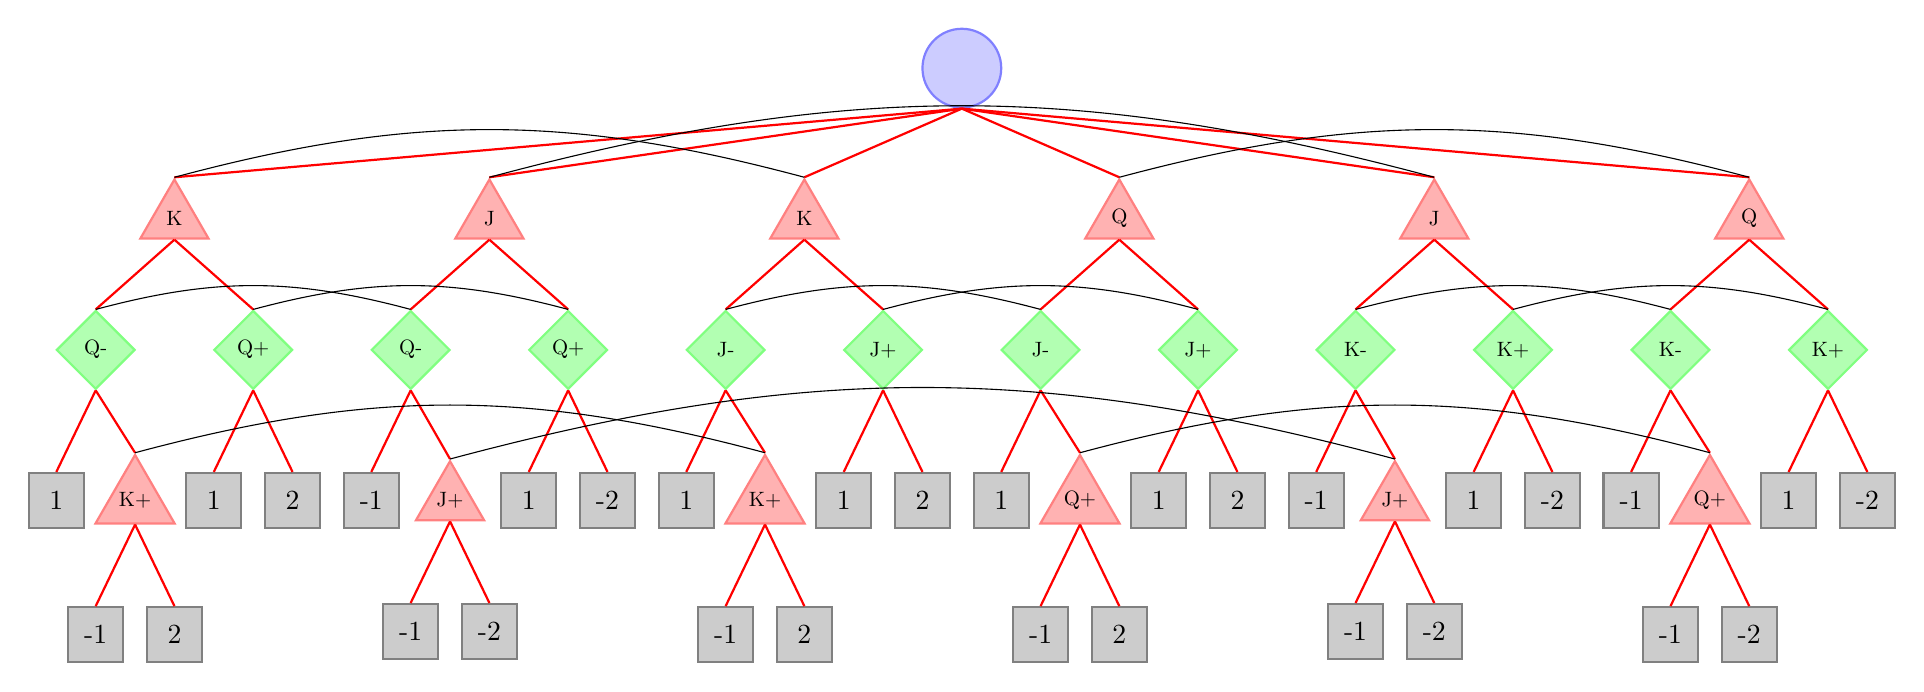
\begin{tikzpicture}
  [chance/.style={circle,draw=blue!50,fill=blue!20,thick,minimum size = 10mm},
   terminal/.style={rectangle,draw=black!50,fill=black!20,thick, minimum size = 7mm},
   maxer/.style={shape=regular polygon, regular polygon sides=3,draw=red!50,fill=red!30,thick,minimum size = 10mm,inner sep = 0pt},
   miner/.style={shape=diamond,draw=green!50,fill=green!30,thick,minimum size = 10mm, inner sep = 0pt},
   edge from parent/.style={red,thick,draw}, 
   parent anchor=south,child anchor=north,
   level 1/.style={sibling distance=4cm,level distance=1.4cm,
       		growth parent anchor=south},
   level 2/.style={sibling distance=2cm},
   level 3/.style={sibling distance=1cm},
   level 4/.style={sibling distance=1.0cm}]
		\node  [chance] {}
		    child {node (M1) [maxer] {\scalebox{.75}{K}}
			child {node (M11) [miner] {\scalebox{.75}{Q-}}
				child {node (M111) [terminal] {1}}
				child {node (M112) [maxer] {\scalebox{.75}{K+}}
					child {node (M1121) [terminal] {-1}}
					child {node (M1122) [terminal] {2}}}
			}
			child {node (M12) [miner] {\scalebox{.75}{Q+}}
				child {node (M121) [terminal] {1}}
				child {node (M122) [terminal] {2}}
			}
		    }
		    child {node (M2) [maxer] {\scalebox{.75}{J}}
			child {node (M21) [miner] {\scalebox{.75}{Q-}}
				child {node (M211) [terminal] {-1}}
				child {node (M212) [maxer] {\scalebox{.75}{J+}}
					child {node (M2121) [terminal] {-1}}
					child {node (M2122) [terminal] {-2}}}
			}
			child {node (M22) [miner] {\scalebox{.75}{Q+}}
				child {node (M221) [terminal] {1}}
				child {node (M222) [terminal] {-2}}
			}
		    }
		    child {node (M3) [maxer] {\scalebox{.75}{K}}
			child {node (M31) [miner] {\scalebox{.75}{J-}}
				child {node (M311) [terminal] {1}}
				child {node (M312) [maxer] {\scalebox{.75}{K+}}
					child {node (M3121) [terminal] {-1}}
					child {node (M3122) [terminal] {2}}}
			}
			child {node (M32) [miner] {\scalebox{.75}{J+}}
				child {node (M321) [terminal] {1}}
				child {node (M322) [terminal] {2}}
			}
		    }
		    child {node (M4) [maxer] {\scalebox{.75}{Q}}
			child {node (M41) [miner] {\scalebox{.75}{J-}}
				child {node (M411) [terminal] {1}}
				child {node (M412) [maxer] {\scalebox{.75}{Q+}}
					child {node (M4121) [terminal] {-1}}
					child {node (M4122) [terminal] {2}}}
			}
			child {node (M42) [miner] {\scalebox{.75}{J+}}
				child {node (M421) [terminal] {1}}
				child {node (M422) [terminal] {2}}
			}
		    }
		    child {node (M5) [maxer] {\scalebox{.75}{J}}
			child {node (M51) [miner] {\scalebox{.75}{K-}}
				child {node (M511) [terminal] {-1}}
				child {node (M512) [maxer] {\scalebox{.75}{J+}}
					child {node (M5121) [terminal] {-1}}
					child {node (M5122) [terminal] {-2}}}
			}
			child {node (M52) [miner] {\scalebox{.75}{K+}}
				child {node (M521) [terminal] {1}}
				child {node (M522) [terminal] {-2}}
			}
		    }
		    child {node (M6) [maxer] {\scalebox{.75}{Q}}
			child {node (M61) [miner] {\scalebox{.75}{K-}}
				child {node (M611) [terminal] {-1}}
				child {node (M612) [maxer] {\scalebox{.75}{Q+}}
					child {node (M6121) [terminal] {-1}}
					child {node (M6122) [terminal] {-2}}}
			}
			child {node (M62) [miner] {\scalebox{.75}{K+}}
				child {node (M621) [terminal] {1}}
				child {node (M622) [terminal] {-2}}
			}
		    };
		\draw  (M1.north) to [dashed,black,out=15,in=165] (M3.north);
		\draw  (M2.north) to [dashed,black,out=15,in=165] (M5.north);
		\draw  (M4.north) to [dashed,black,out=15,in=165] (M6.north);
		\draw  (M112.north) to [dashed,black,out=15,in=165] (M312.north);
		\draw  (M212.north) to [dashed,black,out=15,in=165] (M512.north);
		\draw  (M412.north) to [dashed,black,out=15,in=165] (M612.north);
		\draw  (M11.north) to [dashed,black,out=15,in=165] (M21.north);
		\draw  (M12.north) to [dashed,black,out=15,in=165] (M22.north);
		\draw  (M31.north) to [dashed,black,out=15,in=165] (M41.north);
		\draw  (M32.north) to [dashed,black,out=15,in=165] (M42.north);
		\draw  (M51.north) to [dashed,black,out=15,in=165] (M61.north);
		\draw  (M52.north) to [dashed,black,out=15,in=165] (M62.north);
\end{tikzpicture}
} %scalebox
\caption{}
\label{fulltree}
\end{figure}

Table ~\ref{sampletimes}
\begin{table}
\begin{tabular}{ccc}
1 & 18 & 0.000
2 & 18 & 0.000
3 & 18 & 0.000
4 & 279 & 0.008
5 & 242 & 0.028
6 & 216 & 0.052
7 & 176 & 0.064
8 & 3406 & 0.092
9 & 2191 & 0.288
10 & 1423 & 0.508
11 & 1363 & 0.596
12 & 1416 & 0.744
13 & 1416 & 0.836
14 & 3440 & 0.97
15 & 3428 & 1.25
16 & 50521 & 1.82
17 & 43192 & 5.91
18 & 26128 & 7.94
19 & 19061 & 9.92
\end{tabular}
\caption{Solution counts and running times for a sample kriegspiel game}
\label{white times}
\end{table}

Table ~\ref{sampletimes}
\begin{table}
\begin{tabular}{ccc}
1 & 20 & .000\\
2 & 19 & .000\\
3 & 404 & .008\\
4 & 401 & .024\\
5 & 1472 & .044\\
6 & 155 & .096\\
7 & 293 & .116\\
8 & 158 & .128\\
9 & 118 & .148\\
10 & 25 & .152\\
11 & 798 & .164\\
12 & 518 & .192\\
13 & 13564 & .304\\
14 & 12394 & .776\\
15 & 343652 & 3.75\\
16 & 320704 & 17.345\\
17 & 490162 & 99.9\\
18 & 3792 & 119\\
19 & 14836 & 121 \\
\end{tabular}
\caption{Solution counts and running times for a sample kriegspiel game}
\label{blacktimes}
\end{table}




%\nocite{*}
\nocite{richards09information}
\nocite{russell05efficient}
\nocite{kuhn03lectures}
\nocite{kuhn97classics}
\nocite{parker05sampling}
\nocite{nance06reasoning}
\nocite{li94chess}

\bibliographystyle{acm}
\bibliography{paper}
%\begin{thebibliography}{99}
%\end{thebibliography}

\end{document}
